\chapter{Fluid Picture in Heavy Ion Collisions}

%====================================================================
\section{Bjorken Model}

In a heavy collision, two large nuclei are accelerated to create a head-on collision with a certain impact parameter. Due to the relativistic energies at play both nuclei can be viewed as thin, Lorentz contracted disks of nucleons, that are themselves bound states of quarks, antiquarks and gluons. Therefore, the nuclei form essentially 2-dimensional distributions of these so called parton fields. When the nuclei collide, the strong interaction between the constituents leads to the creation of new QCD matter in the expanding space between the onmoving disks. Due to the strong Lorentz contraction, very high energy densities are achieved initially. It turns out, the system is described fairly accurate by a relativistic fluid, termed the QGP. \todo{Is confinement the right phenomenon to mention here?}.

In a simplified model \cite{Ollitrault_2008} the collision happends almost instantaneously at ${t,z=0}$, $z$ being the coordinate along the collision or beam axis and $t$ the lab time in the center-of-mass frame. If all momentum transfer is localized at this moment of collision, the resulting matter travels along lines of constant ${v_z=z/t}$. Switching into an inertial frame $(t^\prime,z^\prime$) moving longitudinally, i.e. in $z$-direction, with velocity $v$, the change of coordinates from the lab frame $(t,z)$ is mediated by the Lorentz transformation
\begin{equation}
    \begin{pmatrix}
        ct\\z
    \end{pmatrix}
    =
    \begin{pmatrix}
        \gamma&\gamma\beta\\
        \gamma\beta &\gamma
    \end{pmatrix}
    \begin{pmatrix}
        ct^\prime\\
        z
    \end{pmatrix}\,.
\end{equation}
Here we introduced ${\beta=v/c}$ and the relativistic $\gamma$-factor ${\gamma=\sqrt{1-\beta^2}^{-1}}$. We will also make use of the rapidity variable $\eta$, defined by ${\beta=\tanh\eta}$. Whereas ${v_z,z,t}$ change under this boost, the prescription ${v_z=z/t}$ holds both in the old and new inertial frame and is thus boost invariant. In the following we work in units where ${c=1}$

Motivated by empirical data \cite{AlpgardEtAl_1981}, boost invariance as a relevant symmetry was proposed by Bjorken \cite{Bjorken_1983}. He investigated the appearance of a plateau region with respect to rapidity in the spectra of particles produced by nucleon-nucleon and nucleon-nucleus collisions and concluded, that in the mid-rapidity region ${\eta\approx 0}$ initial conditions and therefore also the subsequent dynamics look roughly the same in every reference frame achieved by longitudinal Lorentz boosts or, in other words, that the dynamics are independent of $\eta$. Instead, relevant quantities of the fluid evolution only dependent on proper time ${\tau=\sqrt{t^2-z^2}}$, drastically symplifying all computations.

Whereas the above picture is already sufficient to make significant progress in the treatment of 1-dimensional flow of the QGP, in a real heavy ion collision the spatial extent in the transverse direction, i.e. in the $x$-$y$-plane, of course has to be considered. On one hand, the incoming nuclei need not be aligned perfectly on the collision axis, but are displaced by a certain impact parameter. Accordingly, experimental data is grouped into certain centrality classes. This thesis will focus on central collisions only, which has the benefit that besides longitudinal boost invariance the system is also invariant under azimuthal rotation around the beam axis. On the other hand, the emerging fireball of QGP has finite radius $r$ in transverse direction, such that all evolution equations depend on $\tau$ and $r$ only.

An adapted coordinate system is given in the form of Bjorken- or Milne-coordinates ${(\tau, r, \eta, \varphi)}$, defined by
\begin{equation}
    \left\{\begin{split}
        t&=\tau\cosh\eta\\
        x&=r\cos\varphi\\
        y&=r\sin\varphi\\
        z&=\tau\sinh\eta
    \end{split}\right.
    \qquad\iff\qquad
    \left\{\begin{split}
        \tau&=\sqrt{t^2-z^2}\\
        r&=\sqrt{x^2+y^2}\\
        \eta&=\artanh(z/t)\\
        \varphi&=\arctan(y/x)
    \end{split}\right.\,.
    \label{eq:BjorkenCoords_PositionSpace}
\end{equation}
The Minkwoski metric in these coordinates takes the form ${g_{\mu\nu}=\text{diag}(1,-\tau^2,-1,-r^2)}$. An analogous choice of coordinates can be made in momentum space,
\begin{equation}
    \left\{
    \begin{split}
        p^t&=m_T\cosh\eta_p\\
        p^x&=p_T\cos\varphi_p\\
        p^y&=p_T\sin\varphi_p\\
        p^z&=m_T\sinh\eta_p
    \end{split}
    \right.\qquad\iff\qquad
    \left\{
    \begin{split}
        m_T&=\sqrt{(p^t)^2-(p^z)^2}\\
        p_T&=\sqrt{(p^x)^2+(p^y)^2}\\
        \eta_p&=\artanh(p^z/p^t)\\
        \varphi_p&=\arctan(p^y/p^x)
    \end{split}
    \right.\,.
    \label{eq:BjorkenCoords_MomentumSpace}
\end{equation}
During this thesis, we will encounter contractions of (cartesian) coordinate and momentum vectors ${px\equiv p_\mu x^\mu}$ and ${pq=p_\mu q^\mu}$. Expressed in the curvilinear coordinates given above, they read
\begin{subequations}
    \begin{align}
        p_\mu x^\mu&=-\tau m_T\cosh(\eta-\eta_p)+rp_T\cos(\varphi-\varphi_p)\,,\label{eq:px_contraction}\\
        p_\mu q^\mu&=-m_{T,p}m_{T,q}\cosh(\eta_p-\eta_q)+p_Tq_T\cos(\varphi_p-\varphi_q)\,,\label{eq:pq_contraction}
    \end{align}
    \label{eq:pxpq_contractions}
\end{subequations}
where we used the identities
\begin{equation}
    \cosh(a-b)=\cosh a\cosh b-\sinh a\sinh b\,,\qquad\cos(a-b)=\cos a\cos b+\sin a\sin b\,.
\end{equation}
Note how $x^\mu$ and $p^\mu$ in the new coordinate system are not vector components in a strict sense and cannot be naively contracted using the new metric. The Fourier transform (compare \eqref{eq:FourierConvention})
\begin{equation}
    \tilde{f}(p^\mu)=\int\frac{\dt^4p}{(2\pi)^4}f(x^\mu)\exp\big(-\imagu(\tau m_T\cosh(\eta-\eta_p)-rp_T\cos(\varphi-\varphi_p))\big)
\end{equation}
of a rotationally and boost invariant function ${f(x^\mu)=f(\tau,r)}$ is therefore independent of the $\eta_p$ and $\varphi_p$ momentum components, as can be easily varified by shifting the integration variables ${\eta\to\eta-\eta_p}$ and ${\varphi\to\varphi+\varphi_p}$ in the above integral. The relativistic dispersion relation ${p^2+m^2=0}$ fixes 1 momentum component, typically ${(p^t)^2=\omega_{\vec{p}}^2\equiv m^2+\vec{p}^2}$ in cartesian coordinates or equivalently ${m_T^2=\omega_T^2\equiv m^2+p_T^2}$ in Bjorken coordinates. As we usually work on-shell, i.e. under validity of this dispersion relation, the spectra computed under the above symmetry assumption only depend on transverse momentum, ${\tilde{f}(p^\mu)=\tilde{f}(p_T)}$.



\section{Converting Spectra between Coordinate Systems}
\label{sec:SpectraCoordinateSystem}

In a collider experiment, a number $N$ of particles is counted on the detector. Depending on the detectors capabilities to resolve momentum differences of the incoming particles, the counts are grouped into bins of certain momentum ranges. The continuous analogon of this is to understand the total particle number as an integral over a number density $n(\vec{p})$ and all possible 3-momenta $\vec{p}$,
\begin{equation}
    N=\int\frac{\dt^3p}{(2\pi)^3}n(\vec{p})\,.
    \label{eq:NumberDensity_Cartesian}
\end{equation}
The corresponding 4-momenta $p^\mu$ are chosen to be on-shell for free relativsitic particles and future oriented, $p^t>0$. This definition is intuitive, but not practical given our symmetry assumptions. We shall briefly recapitulate an instructive calculation, showing how to convert spectra between the different coordinate systems.

The total number of particles is conveniently stated as an integral over 4-momenta, enforcing explicitly the dispersion relation and orientation via 
\begin{equation}
    N=2\pi\int\frac{\dt^4p}{(2\pi)^4}\delta(p^2+m^2)\Theta(p^t)\big(2\omega_{\vec{p}}n(\vec{p})\big)\,.
    \label{eq:NumberDensity_4momenta}
\end{equation}
The additional factor of $2\omega_{\vec{p}}$ ensures that the form \eqref{eq:NumberDensity_Cartesian} is restored, after applying the well know identity for the $\delta$-distribution
\begin{equation}
    \delta(f(x))=\sum_{x_i, f(x_i)=0}\frac{\delta(x-x_i)}{\vert f^\prime(x_i)\vert}
\end{equation}
and integrating out the $p^t$-component. The number $N$ of particles counted is the same in any reference frame. Since the integral measure $\dt^4p$ as well as the contraction $p^2$ are Lorentz invariants, it is clear that ${2\omega_{\vec{p}}n(\vec{p})\equiv 2\omega_{\vec{p}}(2\pi)^3(\dt N/\dt^3p)}$ is a Lorentz invariant. On the other hand, we can evaluate the integral \eqref{eq:NumberDensity_4momenta} by performing the change of variables \eqref{eq:BjorkenCoords_PositionSpace}. The Jacobian determinant introduces a factor ${1/m_Tp_T}$ and the $\delta$-distribution cancels the $m_T$-integration, imposing $m_T=\omega_T$. Finally, assuming rotational invariance of the number density, the $\varphi_p$ integration can be performed. Comparing expressions in both coordinate systems, one is lead to the important result
\begin{equation}
    2\omega_{\vec{p}}\frac{\dt N}{\dt p^x\dt p^y\dt p^z}=\frac{1}{2\pi p_T}\frac{\dt N}{\dt p_T\dt \eta_p}\,.
    \label{eq:SpectraConversion}
\end{equation}
Note that this result assumes a symmetry under ${\eta\to-\eta}$, constraining $\eta$ to ${[0,\infty)}$, introducing a factor of $1/2$ on the RHS. If the number density with respect to momentum rapidity ${\eta\in(-\infty,\infty)}$ is considered, one should replace ${2\omega_{\vec{p}}\to\omega_{\vec{p}}}$. Both options are of course Lorentz invariant. More detail is found in the Appendix \ref{sec:Apx_ConvertingSpectra}.



\section{Fundamentals of Relativistic Fluid Dynamics}

If many quantum mechanical particles are involved in the description of a process, finding the exact unitary time evolution of the system state is practically unfeasible. On one hand, explicit analytic expressions for example for eigenstates of the underlying Hamiltonian are rarely accessible, on the other hand numerical algorithms might only scale poorly with the system size, depending on symmetry assumptions etc.

The fundamental idea of thermodynamics is to describe systems of many interacting particles with a set of only a few possibly spacetime dependent variables, such as temperature $T(x)$, particle number $N$, system energy $E$ and volume $V$, among others. To do so, a small number of assumptions and fundamental laws are imposed in order to derive statements about observables of the macroscopic systems and how they arise from a statistical mixture of all possible microscopic states the system could occupy. A crucial part of this is the assumption of thermodynamic equilibrium, meaning a systems extensive parameters do not change. \todo{Work out meaning of equilibrium and out of equilibrium processes}

Based on the ideas of thermodynamics, the field of fluid dynamics tries to predict the collective dynamics of a system of interacting particles.
Dynamics are generated by equations of motion involving the energy-momentum tensor $T^{\mu\nu}(x)$ \cite{Ollitrault_2008},
\begin{equation}
    \begin{split}
        T^{00}\dots\,&\text{energy density,}\\
        T^{0j}\dots\,&\text{$j$th momentum component,}\\
        T^{i0}\dots\,&\text{energy flux in direction $i$,}\\
        T^{ij}\dots\,&\text{flux of $j$th momentum component in direction $i$.}\\
    \end{split}
\end{equation}
It is the conserved current associated to the conservation of 4-momentum, i.e. the symmetry under spacetime translations. \todo{Why does this coincide with the definition $T^{\mu\nu}$ from a Lagrangian?} In a local rest frame the energy-momentum tensor should have the form of static equilibrium \todo{Be specific}. There should be further no flow of particle number or entropy, specifying the form of the particle and entropy current $N^\mu$ and $S^\mu$. In a rest frame one finds
\begin{equation}
    T^{\mu\nu}_{RF}  =
        \begin{pmatrix}
            \epsilon & 0 & 0 & 0 \\
            0        & p & 0 & 0 \\
            0        & 0 & p & 0 \\
            0        & 0 & 0 & p
        \end{pmatrix}\,,\qquad
        N^\mu_{RF}       =
        \begin{pmatrix}
            n\\0\\0\\0
        \end{pmatrix}\,,\qquad
        S^\mu_{RF}       =
        \begin{pmatrix}
            s\\0\\0\\0
        \end{pmatrix}
        \label{eq:FluidMechanics_RestFrame_Quantities}
\end{equation}
with energy density $\epsilon$ and pressure $p$. \todo{Check why kinetic and thermodynamic pressure coincide.} In a general frame these quantitites are obtained by applying a Lorentz boost to \eqref{eq:FluidMechanics_RestFrame_Quantities} and read \cite{Rischke_2022,Weinberg_2008}
\begin{equation}
        T^{\mu\nu}=(\epsilon+p)u^\mu u^\nu+pg^{\mu\nu}\,,\qquad
        N^\mu       =nu^\mu\,,\qquad
        S^\mu       =su^\mu\,,
    \end{equation}
where $u^\mu=(\gamma,\gamma\mathbf{v})$ is the local fluid 4-velocity. Describing wordlines of massive particles, it is a timelike vector, normalized to ${u_\mu u^\mu=-1}$. The term proportional to pressure appearing in the energy momentum tensor is the projector ${\Delta^{\mu\nu}=g^{\mu\nu}+u^\mu u^\nu}$ orthogonal to $u^\mu$. It fulfills
\begin{equation}
    \Delta^{\mu\nu}=\Delta^{\nu\mu}\,,\qquad u_\mu\Delta^{\mu\nu}=0\,,\qquad\Delta^\mu_\lambda\Delta^{\lambda\nu}=\Delta^{\mu\nu}\,\qquad\Delta^\mu_\mu=3=d-1\,.
    \label{eq:FluidMechanics_ProjProperties}
\end{equation}

Local energy-momentum conservation and particle number conservation are encoded by the continuity equations
    \begin{equation}
        \partial_\mu T^{\mu\nu}  =0\,,\qquad
        \partial_\mu N^\mu       =0\,,
    \end{equation}
which constitutes 5 scalar equations for 6 unkwon functions: $\epsilon(x), P(x), n(x), \mathbf{v}(x)$. The equation of state $p=p(\epsilon,n)$ closes the system and captures the characteristics of the matter in question.

\todo{VISCOUS CORRECTIONS}



\subsection{Fluid$\mathbf{u}$M}


\subsection{Blast Wave Model \& Cooper-Frye Freezeout}

A hydrodynamic description can be assumed to be valid until the QGP is so dilute that only few soft scatterings between its components can occur. Thus, there has to be a transition from the fluid regime of the QGP to a regime of free streaming, where particles are considered to be non-interacting.

An intuitive ansatz for this process is given by the so-called Blast Wave model \cite{SiemensRasmussen_1979,FlorkowskiBroniowski_2004,ChenEtAl_2021,JaiswalKoch_2015}. Under radial symmetry, the fireball of QGP is understood as a radial sequence of shells of nuclear matter, the outermost of which experience a stronger accelerating force than the innermost regions due to the drastic gradient in energy density and pressure. This leads to a transverse velocity profile that increases with the radius and an exponential expansion of the fireball. During this expansion, the energy density decreases with increasing surface area, up to a point where kinematic and chemical equilibrium cannot be maintained and the system transitions from collective behaviour to free streaming particles. Drastically simplyfying this gradual process, the Blast Wave model assumes a sharply defined "freezeout" on a fixed codimension-1 hypersurface $\Sigma_{\text{fo}}$ in spacetime, consequently called freezeout surface. Simple models use as this freezeout surface a slice of constant time, constrained by some maximal radius that represents the finite extent of the fireball after a finite evolution time.

The assumption of a freezeout at constant time is of course only an approximation that can be improved upon by more sophisticated treatments of the QGP evolution by fluid models. In general, the freezeout surface for boost and rotationally invariant systems is given by a curve ${\alpha\mapsto\gamma(\alpha)=(\tau(\alpha),r(\alpha))}$, defining the freezeout surface (see figure \ref{fig:FreezeOutSurface_rtau}) with an oriented surface normal $\dt\Sigma^\mu$, see section \ref{sec:FOSurfaceMetric} for details. \todo{Put this or similar image here or later, when deformation of the hypersurfaces is mentioned?}
\debugbox{
    \begin{minipage}{\linewidth}
        \centering
        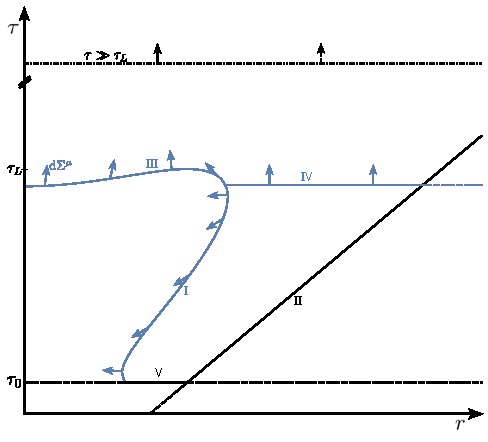
\includegraphics[width=0.5\linewidth]{images/FreezeOutSurface.pdf}
        \captionof{figure}{Freezeout surface in $\tau$-$r$-plane, given by the union $\Sigma_{\rom{1}}/cup\Sigma_{\rom{3}}$ \cite{KirchnerEtAl_2023}.}
        \label{fig:FreezeOutSurface_rtau}
    \end{minipage}
}

The translation from the set of fluid variables to particle spectra is done via the Cooper-Frye freezeout prescription \cite{CooperFrye_1974}
\begin{equation}
    \omega_{\vec{p}}\frac{\dt N}{\dt^3 p}=\frac{1}{(2\pi)^3}\int_\Sigma f(-u_\nu p^\nu)p^\mu\dt\Sigma_\mu\,.
\end{equation}
It assumes that the phase space distribution function $f(x^\mu,p^\nu)$ of particles immediately after freezeout follows a Bose or Fermi distribution plus viscous corrections in the local fluid restframe, that needs to be integrated over the whole freezeout surface in order to find the momentum distribution of all particles produced at freezeout.

Both the hydrodynamic evolution and the freezeout calculation leaves a number of open parameters that are hard to determine from first principles, such as the time $\tau_0$ after which collective hydrodynamic behaviour can be assumed, the temperature at freezeout or viscosity coefficients of the QGP. Being able to efficiently predict particle spectra from a set of parameters allows for a systematic scan over a wide domain in parameter space in order to then find an optimal set of parameters that best characterizes the observed physics. This study was done by the authors of \cite{KirchnerEtAl_2023}.